\documentclass{article}
\usepackage[utf8]{inputenc}
\usepackage[english]{babel}
\usepackage[authoryear,round]{natbib}
\usepackage[colorlinks=true,citecolor=teal, linkcolor=Periwinkle,urlcolor=Periwinkle]{hyperref}
\usepackage[dvipsnames]{xcolor}
\usepackage{graphicx}
\usepackage{amsmath}

\title{Perceptual Losses for Real-Time Style~Transfer and~Super-Resolution}
\author{Iantsa~Provost, Lilian~Rebiere, Bastien~Soucasse, and~Alexey~Zhukov}
\date{January~5, 2022}

\linespread{1.15}
\bibliographystyle{abbrvnat}

\begin{document}

% Title Page
{
    \begin{titlepage}
        \begin{center}
            \vspace*{1.5cm}

            \Large

            \textbf{Perceptual Losses for Real-Time Style~Transfer and~Super-Resolution}

            \vspace{.5cm}

            \vspace{1.5cm}

            \large

            \textbf{Iantsa~Provost, Lilian~Rebiere, Bastien~Soucasse, and~Alexey~Zhukov}

            \vfill

            \normalsize

            Presented as part of the\\
            \textit{AMIP}\\
            course unit.

            \vspace{1.5cm}

            
\includegraphics[width=.5\textwidth]{images/college-logo.jpg}

            Computer~Science~Master's~Degree in~Image~and~Sound\\
            Université~de~Bordeaux,~France\\
            January~5,~2022
        \end{center}
    \end{titlepage}
    \newpage
    \setcounter{page}{2}
}

% Table of Contents
{
    \hypersetup{linkcolor=black}
    \tableofcontents
    \newpage
}

% Introduction
{
    \section{Introduction}
    \label{sec:introduction}

    \cite{sr} introduced a model…

    % Say that we'll only focus on the super resolution part

    % Super-resolution techniques are used to reconstruct high-resolution images from low-resolution versions. These methods have a wide range of applications, including image processing, computer vision, and medical imaging. In this report, we describe the implementation and evaluation of a super resolution model that utilizes perceptual losses. This approach was introduced in the paper "Perceptual Losses for Real-Time Style Transfer and Super-Resolution" by J. Johnson et al. Perceptual losses are designed to capture the high-level features of images and maintain the perceptual quality of the recovered images.

    % To train the model, we used a dataset of high-resolution images. We implemented the model and used this dataset for training.

    % In this report, we present and explain the method used in the model, describe any implementation difficulties that we encountered, and analyze the qualitative and quantitative results of the experiments. We also discuss the energy consumption used during the project and consider other possible impacts. Finally, we suggest possible extensions and future directions for this work.
}

% Method
{
    \section{Method}
    \label{sec:method}

    \begin{figure*}[ht]
        \centering
        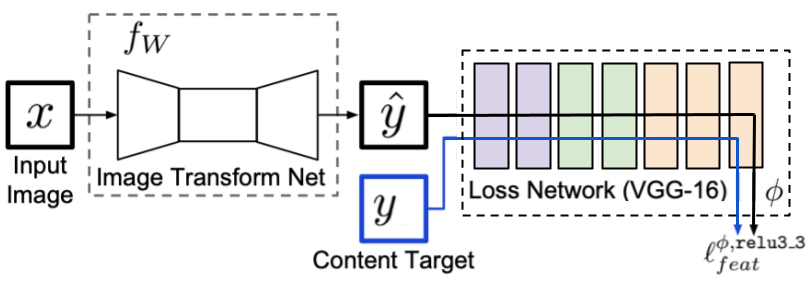
\includegraphics[width=\textwidth]{images/model.png}
        \caption{Overview of the architecture of the proposed model \citep{sr}, focused on the Super-Resolution part.}
        \label{fig:model}
    \end{figure*}

    The proposed model illustrated in Figure~\ref{fig:model} consists of two components: an image transformation network $f_W$ and a loss network $\phi$. Given a low resolution input image $x$, it generates an output image that is expected to be similar to the ground truth high resolution image $y$.

    The image transformation network is a deep residual convolutional neural network with a set of weights parameter denoted $W$. From input images $x$, it provides output images $\hat y$.

    The loss network defines a feature reconstruction loss $l^\phi_{feat}$. It actually delineates several feature reconstruction loss functions $l^{\phi, i}_{feat}(\hat y, y_i)$ that each measures the difference in content between output image $\hat y$ and content target images $y_i$. Here, $i$ denotes the layer.
    % I didn't precise "yc" (which makes the difference with ys for style) because we only measure content difference in our case. Could be modified if you think it's necessary.
    Furthermore, \cite{sr} drew inspiration from several papers such as the one by \cite{gatys} in order to make the most of their feature reconstruction loss. The principle is to use a network pretrained for image classification as a loss network. This way, the beforehand learning of the perceptual and semantic information will facilitate the measure computation of the feature reconstruction loss.

    \bigskip

    Gathering both components, the image transformation network adjusts its weights $W$ by minimizing the combination of those loss functions, using stochastic gradient descent (Equation~\ref{eq:sgd}). Note that the formula given in the paper \citep{sr} mentions a “weighted combination of loss functions” but does not provide more information about the aforementioned weights. As a consequence, we decided to set them all to 1.
    %--it only uses small batch of data to compute the update step at each iteration instead of the average of the gradients in a classic gradient descent.

    \begin{equation}
        W^* =
        \text{argmin}_W \textbf{E}_{x,y_i}
        \biggl[
            \sum_{i=0} l^{\phi, i}_{feat}(f_W(x), y_i)
            \biggr]
        \label{eq:sgd}
    \end{equation}

    \subsection{Image Transfomation Network}
    \label{subsec:image-transform-net}

    % As mentioned previously, the image transformation network is a deep residual convolutional neural network. That is, it includes residual blocks that prevent vanishing gradient issues--when the gradients of the parameters become very small, hindering the ability of the network to learn and improve.

    …

    \subsection{Loss Network}
    \label{subsec:loss-net}

    What propose \cite{sr} is to try and make the images have similar feature representations, instead of forcing a pixel-per-pixel match. To do so and with the intention of making it more performant, the loss network is here defined as a pre-trained network for image classification. More specifically, they use the 16-layer VGG network \citep{vgg} pretrained on the ImageNet dataset \citep{image-net}.

    Now to compute the feature reconstruction loss $l^{\phi, i}_{feat}$ in Equation~\ref{eq:sgd} between the output $\hat y$ and the content target $y$ at a layer $i$, we use the mean square Euclidean distance (Equation~\ref{eq:loss-formula}).

    \begin{equation}
        l^{\phi, i}_{feat}(f_W(x), y_i) =
        \frac{1}{C_i H_i W_i}
        \lVert
        \phi_i (\hat y) - \phi_i (y)
        \rVert_2^2
        \label{eq:loss-formula}
    \end{equation}

    Note that $C_i$, $H_i$ and $W_i$ are respectively the number of channels, height and width of the input image. And, $\phi_i (x)$ is the feature representation of $x$ at layer $i$ (here, $x$ does not mean the input image, but an arbitrary image).
}

% Implementation
{
    \section{Implementation}
    \label{sec:implementation}

    …
}

% Experiments
{
    \section{Experiments}
    \label{sec:experiments}

    \subsection{Setup}
    \label{subsec:setup}

    In order to conduct experiments, we first need a dataset to train our model. \cite{sr} used the MS COCO dataset \citep{mscoco} for training, but due to its large size and the associated training time, we had to find a more adequate dataset.

    As an alternative, we chose DIV2K, a dataset introduced by \cite{div2k_ds} in the technical report \textit{2017 IEEE Conference on Computer Vision and Pattern Recognition Workshops (CVPRW)}. DIV2K is a widely-used dataset for super resolution tasks containing 1000 pairs of low resolution (LR) and high resolution (HR) images. Compared to the MS COCO dataset, it has a reasonable size, making it more feasible for use in this study. More specifically, we only used the HR Images Train Data, which contains 800 images of variable sizes. An extract is visualizable in Figure~\ref{fig:div2k-train-og}.

    \bigskip

    As the model needs a specific type of training data, we did not use the LR images of DIV2K. Indeed, we decided to process the HR images to create our HR-LR pairs. %Furthermore, it allows to store fewer images?

    To do so, the original HR images were cropped to $288 \times 288$ to create the HR patches. Then they were preprocessed according to the methods described in the paper \citep{sr}, to create the LR corresponding patches. It also includes cropping to $288 \times 288$, along with blurring with a Gaussian kernel of width $\sigma = 1.0$, and downsampling with bicubic interpolation.

    Now that the dataset has been preprocessed (see extract in Figure~\\ref{div2k-train-pair}), the model and prepared dataset are now ready to be used for training.

    \begin{figure*}[ht]
        \centering
        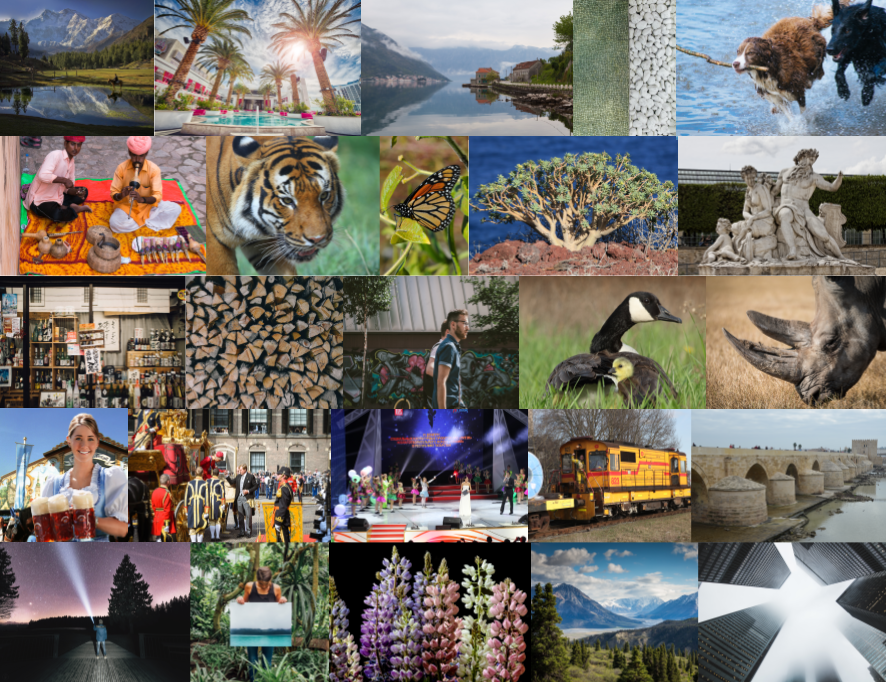
\includegraphics[width=6cm]{images/DIV2K_HR.png}
        \caption{Visualization of 25 DIV2K HR train images.}
        \label{fig:div2k-train-og}
    \end{figure*}

    % \begin{figure*}[ht]
    %     \centering
    %     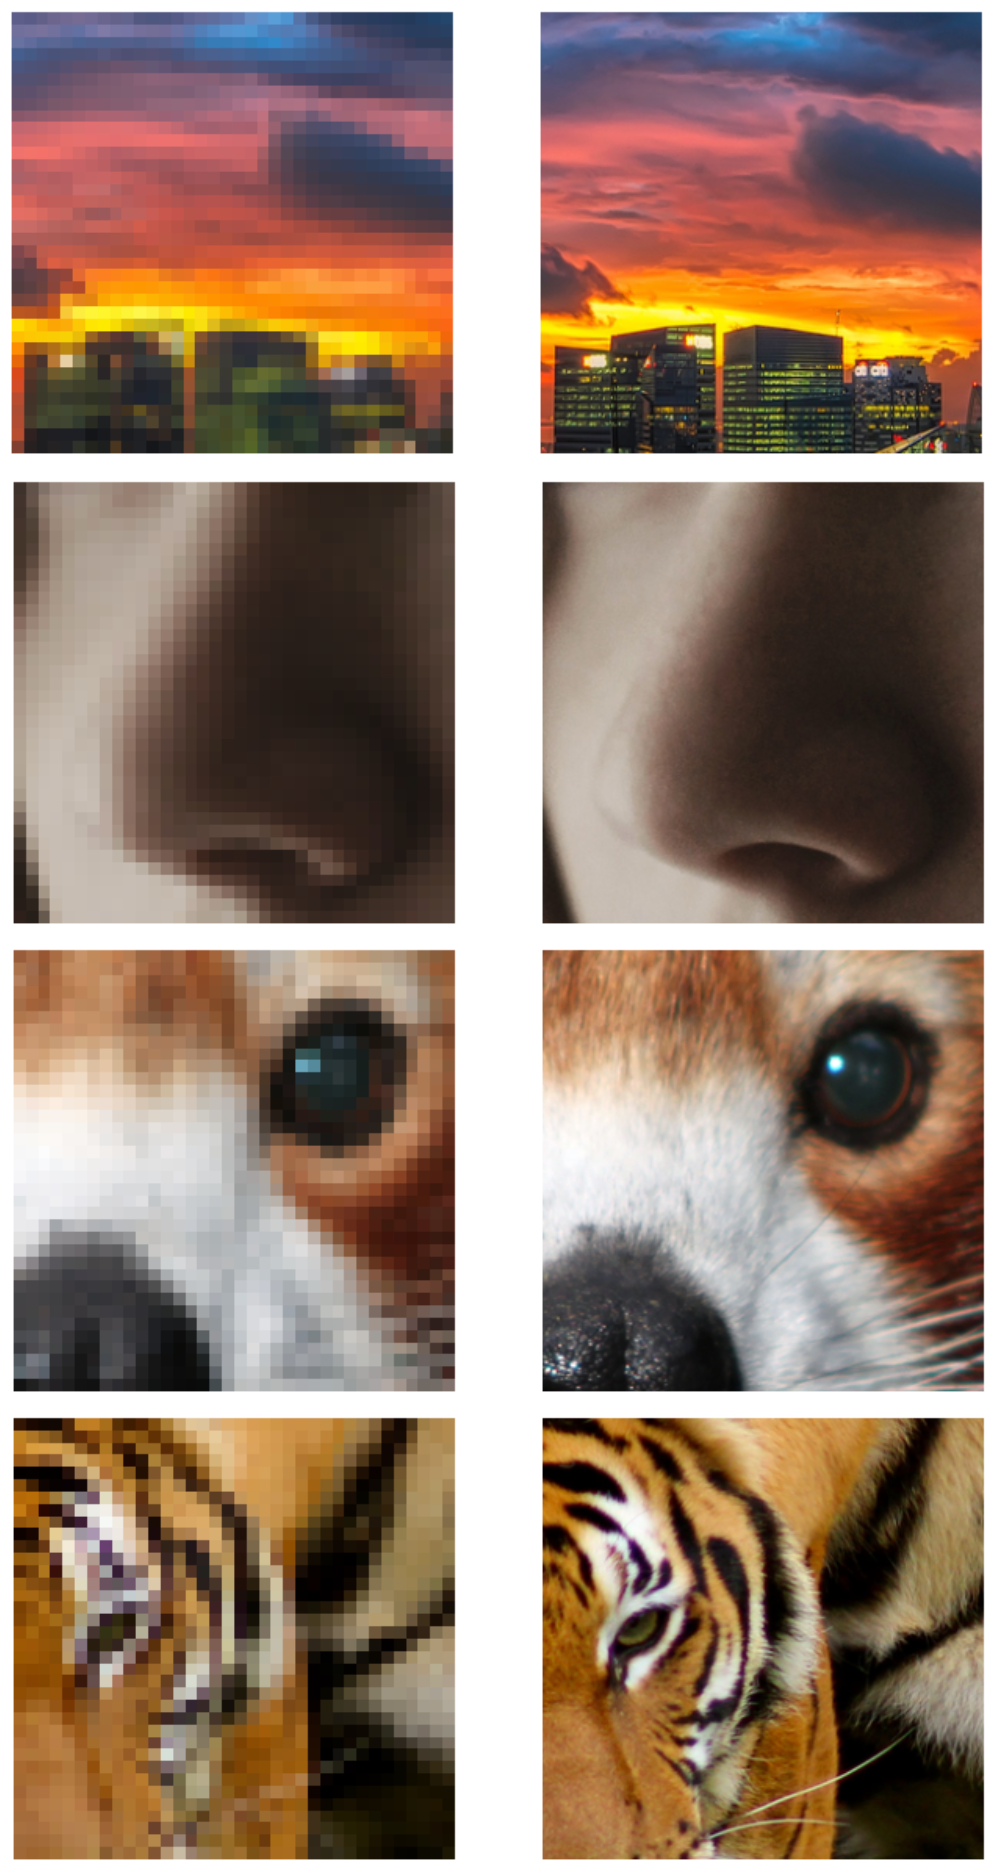
\includegraphics[width=6cm]{images/DIV2K_HRLR.png}
    %     \caption{Visualization of 5 pairs of DIV2K HR train images and their LR corresponding images, that underwent our preprocessing.}
    %     \label{fig:div2k-train-pair}
    % \end{figure*}

    …
}

% Environmental Impact
{
    \section{Environmental Impact}
    \label{sec:env-impact}

    …
}

% Conclusion
{
    \section{Conclusion}
    \label{sec:conclusion}

    …
}

% References
{
    \bibliography{references}
}

\end{document}
